%% This style is provided exclusively for the ICSE 2012 main conference,
%% ICSE 2012 co-located events, and ICSE 2012 workshops.

%% bare_conf_ICSE12.tex
%% V1.4
%% 2012-01-21
%%

%% This is a skeleton file demonstrating the use of IEEEtran.cls
%% (requires IEEEtran.cls version 1.7 or later) with an IEEE conference paper.
%%
%% Support sites:
%% http://www.michaelshell.org/tex/ieeetran/
%% http://www.ctan.org/tex-archive/macros/latex/contrib/IEEEtran/
%% and
%% http://www.ieee.org/

%%*************************************************************************
%% Legal Notice:
%% This code is offered as-is without any warranty either expressed or
%% implied; without even the implied warranty of MERCHANTABILITY or
%% FITNESS FOR A PARTICULAR PURPOSE! 
%% User assumes all risk.
%% In no event shall IEEE or any contributor to this code be liable for
%% any damages or losses, including, but not limited to, incidental,
%% consequential, or any other damages, resulting from the use or misuse
%% of any information contained here.
%%
%% All comments are the opinions of their respective authors and are not
%% necessarily endorsed by the IEEE.
%%
%% This work is distributed under the LaTeX Project Public License (LPPL)
%% ( http://www.latex-project.org/ ) version 1.3, and may be freely used,
%% distributed and modified. A copy of the LPPL, version 1.3, is included
%% in the base LaTeX documentation of all distributions of LaTeX released
%% 2003/12/01 or later.
%% Retain all contribution notices and credits.
%% ** Modified files should be clearly indicated as such, including  **
%% ** renaming them and changing author support contact information. **
%%
%% File list of work: IEEEtran.cls, IEEEtran_HOWTO.pdf, bare_adv.tex,
%%bare_conf.tex, bare_jrnl.tex, bare_jrnl_compsoc.tex
%%*************************************************************************

% *** Authors should verify (and, if needed, correct) their LaTeX system  ***
% *** with the testflow diagnostic prior to trusting their LaTeX platform ***
% *** with production work. IEEE's font choices can trigger bugs that do  ***
% *** not appear when using other class files.***
% The testflow support page is at:
% http://www.michaelshell.org/tex/testflow/



% Note that the a4paper option is mainly intended so that authors in
% countries using A4 can easily print to A4 and see how their papers will
% look in print - the typesetting of the document will not typically be
% affected with changes in paper size (but the bottom and side margins will).
% Use the testflow package mentioned above to verify correct handling of
% both paper sizes by the user's LaTeX system.
%
% Also note that the "draftcls" or "draftclsnofoot", not "draft", option
% should be used if it is desired that the figures are to be displayed in
% draft mode.
%
%% .cls => Style
\documentclass[10pt, conference, compsocconf]{IEEEtran}
% Add the compsocconf option for Computer Society conferences.
%
% If IEEEtran.cls has not been installed into the LaTeX system files,
% manually specify the path to it like:
% \documentclass[conference]{../sty/IEEEtran}
\usepackage[utf8]{inputenc}
%%\usepackage[spanish]{babel}

\usepackage{balance}
\usepackage{url}


% Some very useful LaTeX packages include:
% (uncomment the ones you want to load)


% *** MISC UTILITY PACKAGES ***
%
%\usepackage{ifpdf}
% Heiko Oberdiek's ifpdf.sty is very useful if you need conditional
% compilation based on whether the output is pdf or dvi.
% usage:
% \ifpdf
%   % pdf code
% \else
%   % dvi code
% \fi
% The latest version of ifpdf.sty can be obtained from:
% http://www.ctan.org/tex-archive/macros/latex/contrib/oberdiek/
% Also, note that IEEEtran.cls V1.7 and later provides a builtin
% \ifCLASSINFOpdf conditional that works the same way.
% When switching from latex to pdflatex and vice-versa, the compiler may
% have to be run twice to clear warning/error messages.






% *** CITATION PACKAGES ***
%
%\usepackage{cite}
% cite.sty was written by Donald Arseneau
% V1.6 and later of IEEEtran pre-defines the format of the cite.sty package
% \cite{} output to follow that of IEEE. Loading the cite package will
% result in citation numbers being automatically sorted and properly
% "compressed/ranged". e.g., [1], [9], [2], [7], [5], [6] without using
% cite.sty will become [1], [2], [5]--[7], [9] using cite.sty. cite.sty's
% \cite will automatically add leading space, if needed. Use cite.sty's
% noadjust option (cite.sty V3.8 and later) if you want to turn this off.
% cite.sty is already installed on most LaTeX systems. Be sure and use
% version 4.0 (2003-05-27) and later if using hyperref.sty. cite.sty does
% not currently provide for hyperlinked citations.
% The latest version can be obtained at:
% http://www.ctan.org/tex-archive/macros/latex/contrib/cite/
% The documentation is contained in the cite.sty file itself.






% *** GRAPHICS RELATED PACKAGES ***
%
\ifCLASSINFOpdf
   \usepackage[pdftex]{graphicx}
  % declare the path(s) where your graphic files are
  % \graphicspath{{../pdf/}{../jpeg/}}
  \graphicspath{{./figures/pdf/}{./figures/png/}}
  % and their extensions so you won't have to specify these with
  % every instance of \includegraphics
   \DeclareGraphicsExtensions{.pdf,.jpeg,.png}
\else
  % or other class option (dvipsone, dvipdf, if not using dvips). graphicx
  % will default to the driver specified in the system graphics.cfg if no
  % driver is specified.
  % \usepackage[dvips]{graphicx}
  \usepackage[dvipdf]{graphicx}
  % declare the path(s) where your graphic files are
   \graphicspath{{./figures/eps/}}
  % and their extensions so you won't have to specify these with
  % every instance of \includegraphics
   \DeclareGraphicsExtensions{.eps}
\fi
% graphicx was written by David Carlisle and Sebastian Rahtz. It is
% required if you want graphics, photos, etc. graphicx.sty is already
% installed on most LaTeX systems. The latest version and documentation can
% be obtained at: 
% http://www.ctan.org/tex-archive/macros/latex/required/graphics/
% Another good source of documentation is "Using Imported Graphics in
% LaTeX2e" by Keith Reckdahl which can be found as epslatex.ps or
% epslatex.pdf at: http://www.ctan.org/tex-archive/info/
%
% latex, and pdflatex in dvi mode, support graphics in encapsulated
% postscript (.eps) format. pdflatex in pdf mode supports graphics
% in .pdf, .jpeg, .png and .mps (metapost) formats. Users should ensure
% that all non-photo figures use a vector format (.eps, .pdf, .mps) and
% not a bitmapped formats (.jpeg, .png). IEEE frowns on bitmapped formats
% which can result in "jaggedy"/blurry rendering of lines and letters as
% well as large increases in file sizes.
%
% You can find documentation about the pdfTeX application at:
% http://www.tug.org/applications/pdftex

%\usepackage{graphicx}




% *** MATH PACKAGES ***
%
%\usepackage[cmex10]{amsmath}
% A popular package from the American Mathematical Society that provides
% many useful and powerful commands for dealing with mathematics. If using
% it, be sure to load this package with the cmex10 option to ensure that
% only type 1 fonts will utilized at all point sizes. Without this option,
% it is possible that some math symbols, particularly those within
% footnotes, will be rendered in bitmap form which will result in a
% document that can not be IEEE Xplore compliant!
%
% Also, note that the amsmath package sets \interdisplaylinepenalty to 10000
% thus preventing page breaks from occurring within multiline equations. Use:
%\interdisplaylinepenalty=2500
% after loading amsmath to restore such page breaks as IEEEtran.cls normally
% does. amsmath.sty is already installed on most LaTeX systems. The latest
% version and documentation can be obtained at:
% http://www.ctan.org/tex-archive/macros/latex/required/amslatex/math/





% *** SPECIALIZED LIST PACKAGES ***
%
%\usepackage{algorithmic}
% algorithmic.sty was written by Peter Williams and Rogerio Brito.
% This package provides an algorithmic environment fo describing algorithms.
% You can use the algorithmic environment in-text or within a figure
% environment to provide for a floating algorithm. Do NOT use the algorithm
% floating environment provided by algorithm.sty (by the same authors) or
% algorithm2e.sty (by Christophe Fiorio) as IEEE does not use dedicated
% algorithm float types and packages that provide these will not provide
% correct IEEE style captions. The latest version and documentation of
% algorithmic.sty can be obtained at:
% http://www.ctan.org/tex-archive/macros/latex/contrib/algorithms/
% There is also a support site at:
% http://algorithms.berlios.de/index.html
% Also of interest may be the (relatively newer and more customizable)
% algorithmicx.sty package by Szasz Janos:
% http://www.ctan.org/tex-archive/macros/latex/contrib/algorithmicx/




% *** ALIGNMENT PACKAGES ***
%
%\usepackage{array}
% Frank Mittelbach's and David Carlisle's array.sty patches and improves
% the standard LaTeX2e array and tabular environments to provide better
% appearance and additional user controls. As the default LaTeX2e table
% generation code is lacking to the point of almost being broken with
% respect to the quality of the end results, all users are strongly
% advised to use an enhanced (at the very least that provided by array.sty)
% set of table tools. array.sty is already installed on most systems. The
% latest version and documentation can be obtained at:
% http://www.ctan.org/tex-archive/macros/latex/required/tools/


%\usepackage{mdwmath}
%\usepackage{mdwtab}
% Also highly recommended is Mark Wooding's extremely powerful MDW tools,
% especially mdwmath.sty and mdwtab.sty which are used to format equations
% and tables, respectively. The MDWtools set is already installed on most
% LaTeX systems. The lastest version and documentation is available at:
% http://www.ctan.org/tex-archive/macros/latex/contrib/mdwtools/


% IEEEtran contains the IEEEeqnarray family of commands that can be used to
% generate multiline equations as well as matrices, tables, etc., of high
% quality.


%\usepackage{eqparbox}
% Also of notable interest is Scott Pakin's eqparbox package for creating
% (automatically sized) equal width boxes - aka "natural width parboxes".
% Available at:
% http://www.ctan.org/tex-archive/macros/latex/contrib/eqparbox/





% *** SUBFIGURE PACKAGES ***
%\usepackage[tight,footnotesize]{subfigure}
% subfigure.sty was written by Steven Douglas Cochran. This package makes it
% easy to put subfigures in your figures. e.g., "Figure 1a and 1b". For IEEE
% work, it is a good idea to load it with the tight package option to reduce
% the amount of white space around the subfigures. subfigure.sty is already
% installed on most LaTeX systems. The latest version and documentation can
% be obtained at:
% http://www.ctan.org/tex-archive/obsolete/macros/latex/contrib/subfigure/
% subfigure.sty has been superceeded by subfig.sty.



%\usepackage[caption=false]{caption}
%\usepackage[font=footnotesize]{subfig}
% subfig.sty, also written by Steven Douglas Cochran, is the modern
% replacement for subfigure.sty. However, subfig.sty requires and
% automatically loads Axel Sommerfeldt's caption.sty which will override
% IEEEtran.cls handling of captions and this will result in nonIEEE style
% figure/table captions. To prevent this problem, be sure and preload
% caption.sty with its "caption=false" package option. This is will preserve
% IEEEtran.cls handing of captions. Version 1.3 (2005/06/28) and later 
% (recommended due to many improvements over 1.2) of subfig.sty supports
% the caption=false option directly:
%\usepackage[caption=false,font=footnotesize]{subfig}
%
% The latest version and documentation can be obtained at:
% http://www.ctan.org/tex-archive/macros/latex/contrib/subfig/
% The latest version and documentation of caption.sty can be obtained at:
% http://www.ctan.org/tex-archive/macros/latex/contrib/caption/




% *** FLOAT PACKAGES ***
%
%\usepackage{fixltx2e}
% fixltx2e, the successor to the earlier fix2col.sty, was written by
% Frank Mittelbach and David Carlisle. This package corrects a few problems
% in the LaTeX2e kernel, the most notable of which is that in current
% LaTeX2e releases, the ordering of single and double column floats is not
% guaranteed to be preserved. Thus, an unpatched LaTeX2e can allow a
% single column figure to be placed prior to an earlier double column
% figure. The latest version and documentation can be found at:
% http://www.ctan.org/tex-archive/macros/latex/base/



%\usepackage{stfloats}
% stfloats.sty was written by Sigitas Tolusis. This package gives LaTeX2e
% the ability to do double column floats at the bottom of the page as well
% as the top. (e.g., "\begin{figure*}[!b]" is not normally possible in
% LaTeX2e). It also provides a command:
%\fnbelowfloat
% to enable the placement of footnotes below bottom floats (the standard
% LaTeX2e kernel puts them above bottom floats). This is an invasive package
% which rewrites many portions of the LaTeX2e float routines. It may not work
% with other packages that modify the LaTeX2e float routines. The latest
% version and documentation can be obtained at:
% http://www.ctan.org/tex-archive/macros/latex/contrib/sttools/
% Documentation is contained in the stfloats.sty comments as well as in the
% presfull.pdf file. Do not use the stfloats baselinefloat ability as IEEE
% does not allow \baselineskip to stretch. Authors submitting work to the
% IEEE should note that IEEE rarely uses double column equations and
% that authors should try to avoid such use. Do not be tempted to use the
% cuted.sty or midfloat.sty packages (also by Sigitas Tolusis) as IEEE does
% not format its papers in such ways.





% *** PDF, URL AND HYPERLINK PACKAGES ***
%
%\usepackage{url}
% url.sty was written by Donald Arseneau. It provides better support for
% handling and breaking URLs. url.sty is already installed on most LaTeX
% systems. The latest version can be obtained at:
% http://www.ctan.org/tex-archive/macros/latex/contrib/misc/
% Read the url.sty source comments for usage information. Basically,
% \url{my_url_here}.





% *** Do not adjust lengths that control margins, column widths, etc. ***
% *** Do not use packages that alter fonts (such as pslatex). ***
% There should be no need to do such things with IEEEtran.cls V1.6 and later.
% (Unless specifically asked to do so by the journal or conference you plan
% to submit to, of course. )


% correct bad hyphenation here
\hyphenation{op-tical net-works semi-conduc-tor}


\begin{document}
%
% paper title
% can use linebreaks \\ within to get better formatting as desired
\title{The influence of bug subscribers on the development of Android}


% author names and affiliations
% use a multiple column layout for up to two different
% affiliations

\author{
\IEEEauthorblockN{Antonio Arias Losada}
\IEEEauthorblockA{ Master on Free Software 2012, Vigo Edition\\
Pontevedra, Spain\\
antonio.arias@gmail.com}
\and

\IEEEauthorblockN{Francisco Alberto Rocha Rivera}
\IEEEauthorblockA{Master on Free Software 2012, Vigo Edition\\
Vigo, Spain\\
rocha.francisco.a@gmail.com}
}

% conference papers do not typically use \thanks and this command
% is locked out in conference mode. If really needed, such as for
% the acknowledgment of grants, issue a \IEEEoverridecommandlockouts
% after \documentclass

% for over three affiliations, or if they all won't fit within the width
% of the page, use this alternative format:
% 
%\author{\IEEEauthorblockN{Michael Shell\IEEEauthorrefmark{1},
%Homer Simpson\IEEEauthorrefmark{2},
%James Kirk\IEEEauthorrefmark{3}, 
%Montgomery Scott\IEEEauthorrefmark{3} and
%Eldon Tyrell\IEEEauthorrefmark{4}}
%\IEEEauthorblockA{\IEEEauthorrefmark{1}School of Electrical and Computer Engineering\\
%Georgia Institute of Technology,
%Atlanta, Georgia 30332--0250\\ Email: see http://www.michaelshell.org/contact.html}
%\IEEEauthorblockA{\IEEEauthorrefmark{2}Twentieth Century Fox, Springfield, USA\\
%Email: homer@thesimpsons.com}
%\IEEEauthorblockA{\IEEEauthorrefmark{3}Starfleet Academy, San Francisco, California 96678-2391\\
%Telephone: (800) 555--1212, Fax: (888) 555--1212}
%\IEEEauthorblockA{\IEEEauthorrefmark{4}Tyrell Inc., 123 Replicant Street, Los Angeles, California 90210--4321}}




% use for special paper notices
%\IEEEspecialpapernotice{(Invited Paper)}




% make the title area
\maketitle


\begin{abstract}
The Android bug tracking system has a subscribing mechanism whose
purpose is to let the developers learn about the importance of a
particular bug for the users of the operating system. This mechanism
scores a star to a bug each time a user subscribes to that particular
bug. In this MSR challenge report we try to find how that mechanism
influences the way the developers prioritize the resolution of a bug,
either by giving the bug a higher priority or by resolving the bug
faster. We study the time to close bugs reported in the public Android
BTS, as well as the priority of the bugs, trying to relate each of
those variables with the number of subscribers of the bugs. The
results show that most of the bugs have the same priority, and that
the resolution time is not influenced by the number of stars. We
analyze why this is happening and conclude that there is no relation
neither between the number of stars of a bug and the time it requires to be solved, nor between the number of stars of a bug and the priority the developers assign to the bug.
\end{abstract}

\begin{IEEEkeywords}
Android, MSR challenge, bug tracking system, BTS, subscribers, stars, priority, bug resolution time
%%component; formatting; style; styling
\end{IEEEkeywords}


% For peer review papers, you can put extra information on the cover
% page as needed:
% \ifCLASSOPTIONpeerreview
% \begin{center} \bfseries EDICS Category: 3-BBND \end{center}
% \fi
%
% For peerreview papers, this IEEEtran command inserts a page break and
% creates the second title. It will be ignored for other modes.
\IEEEpeerreviewmaketitle



\section{Introduction}
%%\url {http://2012.msrconf.org/challenge.php}.
Bug reporting is an essential component of the development model of an open source project. Testing and validation of the project is mainly performed by users, who can contribute back to the project by reporting bugs. The more users inspecting and testing the code of a project, the quickest any bug will be located and the more probable is that someone finds a fix for the bug (Linus' Law \cite{CathedralBazaar}). Therefore, bug tracking systems (BTS) are essential for the management and growth of open source projects, allowing direct and organized communication between users and developers of the project.

The bug tracker plays a crucial role on the development of the project as it centralizes development requests. But from the point of view of project planning, the tracker presents a big challenge because of the large amount of information gathered. Prioritizing all that information is fundamental for the definition of the roadmap of the project. The developers need to classify the bugs according to some criteria in order to generate a prioritized list of pending tasks, given that it is impossible to solve all the bugs as they are being reported.

In order to do that classification, the number of users interested in a particular bug should be a good measure of the relevance of the bug and, by extension, a measure of the importance of that bug for the developers of the project. To help cope with this issue, some bug tracking systems incorporate a mechanism which lets users subscribe to bugs, and thus enable a mechanism for prioritizing them. This is the case of Android. Like most open source projects do, the Android project maintains a public bug tracker where users can report bugs and request features for the Android software stack, as well as subscribe to bugs. As stated by the Android bug tracker \cite{ReportBugs}, the number of users subscribed to a bug influences the way developers prioritize the bug. We would like to know if the mechanism is actually effective and working as expected.

From the moment a bug is reported, up until it is closed, the bug may be in different states of progress. The current state is tracked through a status assigned to the bug. Bug reporters and members of the community are allowed to subscribe to any particular bug in order to be notified by mail each time the status of the bug is changed.  For each bug, the tracker keeps a metric named stars. A star is scored to a bug each time a user subscribes to the state of the bug. Thus the number of stars of a bug is equivalent to the number of members of the community that have explicitly shown interest on the state of that particular bug. When reporting a bug or  while browsing the reported issues, the users click on a star-shaped check box in order to subscribe to a bug. Hence the name of the metric. This information is reported in the tracker documentation to be considered by the developers in order to prioritize the resolution of the bugs, so the developers are expected to attend first those bugs with more subscribers, that is, the ones which have more relevance for the community.

We believe that if developers take into account the number of subscribers of a bug for the development of the project, then we should observe some relation between the number of stars of a bug and the time that bug takes to be solved. We should also expect to see a relation between the priority of a bug and the number of stars of that particular bug. The objective of this paper is to evaluate these two statements using the bug reports provided in XML format by the MSR 2012 challenge \cite{MSR} 

The rest of this paper is organized as follows: the next section describes work related to this project. Section III provides both the data source and the statistical analysis used in this study, while Section IV presents our results. Section V presents a discussion about conditions that constrain our results. The last section includes conclusions and some considerations for further work.

\section{Related Research}
The influence of the subscribers of bugs on Open Source projects has not been studied thoroughly. However there are some works that have related the resolution time of bugs with other parameters. Herraiz et al \cite{EclipseSimplification} studied the mean time to close bugs reported in Eclipse, and related it to how the severity assigned by users affects this time. In particular, the study classifies bugs according to the time it takes to solve them, grouping the results in severity categories. Crowston et al \cite{Portfolio} have also studied bug fixing time as a measure of FLOSS projects success, entering bug priority as a factor of the study. The paper presents a statistical analysis of the time to close bugs modeled as censored data.

\section{Methodology}

\subsection {Data gathering}
%\emph{BTS Data}
We have made the current study from the data provided for the Mining Challenge of the 9th International Working Conference on Mining Software Repositories (MSR) \cite{MSR}. Specifically, we have extracted the needed information from the bugs reported on the tracker of the project, provided in XML format.

We developed a Java application to parse the XML document containing the bug information by means of the StAX API (Streaming API for XML) \cite{StAX}. Traditionally XML APIs are either DOM based, which support random access but are very resource consuming, or event based, which are very efficient but not very user-friendly. The StAX API is designed to close the gap between those two approaches. This API allowed us to cope with the big XML document provided for the challenge (2GB) efficiently and effectively.

We only included closed bugs. For each bug we evaluated the required time to be solved, computing it from the bug opening and closing timestamps provided in the bug document. We converted their timestamps into UTC seconds. Subtracting the values corresponding to the closing and opening timestamps we obtained the number of seconds invested to solve the bug. The resolution is the minimum we considered appropriate, since the bug that required less time took 17 seconds to be solved. The resulting application parses the bugs and exports the number of stars of that bug, its priority and the number of seconds that the bug required to be fixed to a text file. This file allowed us to import the data into a GNU R \cite{WhatIsR} environment in order to process it. GNU R is a free software environment for statistical computing and graphics. It provides a wide variety of statistical and graphical techniques, so it fulfilled our statistical and graphic needs for the present study \cite{RNutshell}. Once we had the data we needed imported into GNU R, we applied the methodology presented on the next section.

\subsection {Statistical Analysis}
We are trying to validate two hypotheses, (1) the time required to solve a particular bug has some statistical dependence with the number of subscribers of the bug, and (2) the priority assigned by the developers to a particular bug has some statistical dependence with the number of subscribers of the bug.

In order to validate the first of our hypothesis, first of all we analyzed the boxplot of the times to close  bugs and the number of subscribers, in order to have a quick evaluation of the ranges of the variables. Then we grouped the bugs by number of subscribers in order to study the relation between number of subscribers and resolution time. We discarded the possibility of evaluating the mean length of time required to close bugs with a particular number of subscribers, because not all the values for every number of subscribers have the same number of bugs, so the average values are skewed. Therefore we studied the resolution times for all the bugs instead of studying only the mean values for the bugs that share the same number of subscribers. In any case, we also computed the medians for the resolution times, which gave us a more robust view of the resolution times.
Our study is based on the iteration over possible statistical relations in order to find the influence of the number of subscribers on the resolution time of the bugs.

We evaluate the density function of the logarithm of the number of subscribers of the bugs in order to deduce a possible statistical distribution.  

Then we analyzed the cumulative distribution function of the resolution time. In particular, we use the inverse of the cumulative distribution function, because cognitive psychology tells that it is easier to discern variations on descent curves  \cite{NowYouSeeIt}.

We also tried to approximate the distribution of the samples with a Poisson distribution and repeated the process with an exponential distribution.

Finally we computed the value of the correlation between the resolution time and the number of subscribers of the bugs. We computed the Pearson coefficient, which measures linear correlation, as well as both Kendall and Spearman coefficients, which measure if there is any kind of strong relation between both variables, even if it is not linear.

In order to validate our second hypotheses, we have also tried to relate a bug priority with its number of subscribers in a analogous way as we did with the bug resolution time.

\section{Results}
%\includegraphics{figures/stars-duration-log.png}
According to the Android BTS \cite{ReportBugs}, the number of subscribers of a bug helps developers know which bugs are more relevant for the community. \ref{fig:stars-duration} represents the time to solve bugs. The horizontal axis represents the number of subscribers of a bug, while the values on the vertical axis represent the time to close bugs. In order to increase resolution, both axes are presented in logarithmic scale. Given the variability on the vertical axis, we can see that the time to close a bug is not influenced by the number of subscribers of the bug.


The existence of a large number of bugs with a single star seems to reflect the fact that the community is not involved in the bug subscription mechanism. Moreover, there is a large amount of bugs with just a single subscriber. It should be noted that when a bug is reported, by default the reporter of the bug is subscribed to it (logically it is assumed the interest of the reporters on the bugs they report). 

We have found no statistical relation between the number of subscribers and the resolution time of the bugs by evaluating density functions and cumulative distributions. Correlation coefficients also show no statistical dependency between both variables.

We suppose that the number of  subscribers of a bug is somehow used by the developers to assign the priority value of each bug. We have represented the priorities against the number of subscribers. The results are shown in \ref{fig:stars-priority}. The horizontal axis represents the number of subscribers of a bug, while the values on the vertical axis represent the priority of the bugs. The figure shows that almost all bugs have “Medium” priority, which seems to portray the fact that developers do not pay special attention to this property.

All the above seems the true reflection of the closed contribution model of the Android development approach and the fact that Google takes all the decisions regarding the operating system unilaterally. The release cycle makes the source code public only after releasing binaries. 

\begin{figure}[!t]
\centering
\includegraphics[width=2.5in]{stars-duration-log}
\caption{Bug resolution time}
\label{fig:stars-duration}
\end{figure}

\begin{figure}[!t]
\centering
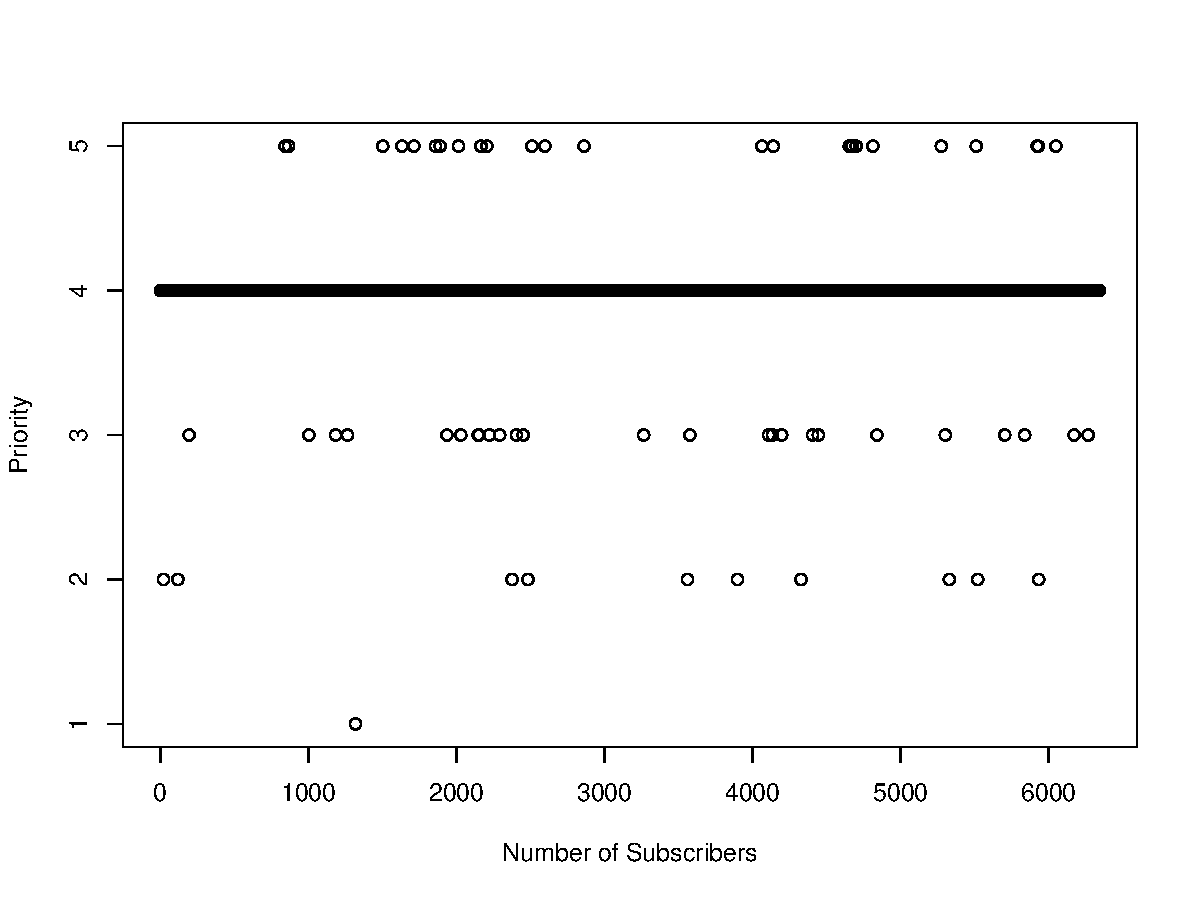
\includegraphics[width=2.5in]{stars-priority}
\caption{Bug priority}
\label{fig:stars-priority}
\end{figure}

\section{Threats to validity}
Our model is based on features that can easily be gathered from bug report submissions. Construct validity requires that we correctly identify resolution time, number of subscribers and priority for each bug of the project. These are straightforward values directly obtained by simple arithmetic calculations from the information provided by the tracker.

The main threat to the external validity of our study is the actual veracity of the values provided by the tracker. There are several systems keeping track of the bugs of the operating system, among which some are kept private by Google \cite{LifeBug}. This means that the information of the public tracker is partial and incomplete, as reflected by the fact that the majority of the bugs present the same priority. That compromises the validity of our study, but in no case prevents our method to be applied to any other set of data.

We have not classified a sample from the data, but taken all the bugs stored in the database to make the analysis. This approach may suppose some threats to the validity of the analysis, because not all the components of the operating system have the same interest for the community. Furthermore, not all the components have the same number of users capable of detecting their bugs. For example, it is not as usual to spot a bug on the Dalvik virtual machine than it is to do it on the Gmail application. Moreover, in a mainstream project like Android it must be taken into account that not all the users of the operating system are reflected in the bug tracker, as most of them are not even aware of its existence and purpose. Our study may be repeated filtering the different bugs by component (Dalvik, Tools, Applications, etc.) thus selecting the size and properties of the sample in order to be more precise.

It is not possible to link the information present on the bug tracker with the information on the code repositories, so we could not apply any metric regarding the code (lines, comments, committers) in order to improve our study.

%\section{Further Work}
%TBD

\section{Conclusions and Further Work}
Almost all bugs registered in the public Android tracker have the same priority and there is no relation between the resolution time and the number of subscribers of the bugs.

As stated by the Android Open Source Project, there are several trackers for the bugs of the operating system, among which only the studied tracker is official and public. This is a major determinant for the results of our study. The information of the public tracker is distorted because the actual development is driven by the private tracker, as reflected by the fact that almost all bugs share the same priority. We may deduce that the priorities of the bugs are actually tracked by the private tracker and never reflected back to the public tracker. We also believe that the number of subscribers of a bug is not a major factor in the prioritization made by the developers.

Regarding the relation between the resolution time and the number of subscribers of a bug, there are also many other factors that come into play. For example, a bug that might have more relevance for the community can be solved faster because it is not very complex or has high private priority, thus not spending enough time open to build up a large number of stars. In contrast, a bug that is less relevant for the community may stay open more time, either because it is very complex or has low private priority, making it easier for the bug to accumulate more stars during its life.

We would like to have access to the private bug tracker databases of the project in order to evaluate their information, apply the presented statistical analysis and compare the results with the ones we have found here. However, bug tracking systems databases not always are available to researches and third parties, especially those related with OEMs. This issue is even more evident in the case of Google, which not only keeps a private bug tracking system, but also keeps the development private, making the source code available to the community only after releasing binaries. Making the information of the development available would help better  understand the dynamics of the project.



%\url{ http://www.ifi.uzh.ch/icse2012/how-to-submit/ }
%Inside 2012.msrconf.org 

% An example of a floating figure using the graphicx package.
% Note that \label must occur AFTER (or within) \caption.
% For figures, \caption should occur after the \includegraphics.
% Note that IEEEtran v1.7 and later has special internal code that
% is designed to preserve the operation of \label within \caption
% even when the captionsoff option is in effect. However, because
% of issues like this, it may be the safest practice to put all your
% \label just after \caption rather than within \caption{}.
%
% Reminder: the "draftcls" or "draftclsnofoot", not "draft", class
% option should be used if it is desired that the figures are to be
% displayed while in draft mode.
%
%\begin{figure}[!t]
%\centering
%\includegraphics[width=2.5in]{myfigure}
% where an .eps filename suffix will be assumed under latex, 
% and a .pdf suffix will be assumed for pdflatex; or what has been declared
% via \DeclareGraphicsExtensions.
%\caption{Simulation Results}
%\label{fig_sim}
%\end{figure}

% Note that IEEE typically puts floats only at the top, even when this
% results in a large percentage of a column being occupied by floats.


% An example of a double column floating figure using two subfigures.
% (The subfig.sty package must be loaded for this to work.)
% The subfigure \label commands are set within each subfloat command, the
% \label for the overall figure must come after \caption.
% \hfil must be used as a separator to get equal spacing.
% The subfigure.sty package works much the same way, except \subfigure is
% used instead of \subfloat.
%
%\begin{figure*}[!t]
%\centerline{\subfloat[Case I]\includegraphics[width=2.5in]{subfigcase1}%
%\label{fig_first_case}}
%\hfil
%\subfloat[Case II]{\includegraphics[width=2.5in]{subfigcase2}%
%\label{fig_second_case}}}
%\caption{Simulation results}
%\label{fig_sim}
%\end{figure*}
%
% Note that often IEEE papers with subfigures do not employ subfigure
% captions (using the optional argument to \subfloat), but instead will
% reference/describe all of them (a), (b), etc., within the main caption.


% An example of a floating table. Note that, for IEEE style tables, the 
% \caption command should come BEFORE the table. Table text will default to
% \footnotesize as IEEE normally uses this smaller font for tables.
% The \label must come after \caption as always.
%
%\begin{table}[!t]
%% increase table row spacing, adjust to taste
%\renewcommand{\arraystretch}{1.3}
% if using array.sty, it might be a good idea to tweak the value of
% \extrarowheight as needed to properly center the text within the cells
%\caption{An Example of a Table}
%\label{table_example}
%\centering
%% Some packages, such as MDW tools, offer better commands for making tables
%% than the plain LaTeX2e tabular which is used here.
%\begin{tabular}{|c||c|}
%\hline
%One & Two\\
%\hline
%Three & Four\\
%\hline
%\end{tabular}
%\end{table}


% Note that IEEE does not put floats in the very first column - or typically
% anywhere on the first page for that matter. Also, in-text middle ("here")
% positioning is not used. Most IEEE journals/conferences use top floats
% exclusively. Note that, LaTeX2e, unlike IEEE journals/conferences, places
% footnotes above bottom floats. This can be corrected via the \fnbelowfloat
% command of the stfloats package.




% use section* for acknowledgement
%\section*{Acknowledgment}


% trigger a \newpage just before the given reference
% number - used to balance the columns on the last page
% adjust value as needed - may need to be readjusted if
% the document is modified later
%\IEEEtriggeratref{8}
% The "triggered" command can be changed if desired:
%\IEEEtriggercmd{\enlargethispage{-5in}}

% Better way for balancing the last page:

\balance

% references section

% can use a bibliography generated by BibTeX as a .bbl file
% BibTeX documentation can be easily obtained at:
% http://www.ctan.org/tex-archive/biblio/bibtex/contrib/doc/
% The IEEEtran BibTeX style support page is at:
% http://www.michaelshell.org/tex/ieeetran/bibtex/
%\bibliographystyle{IEEEtran}
% argument is your BibTeX string definitions and bibliography database(s)
%\bibliography{IEEEabrv,../bib/paper}
%
% <OR> manually copy in the resultant .bbl file
% set second argument of \begin to the number of references
% (used to reserve space for the reference number labels box)
%\begin{thebibliography}{1}
%
%\bibitem{IEEEhowto:kopka}
%H.~Kopka and P.~W. Daly, \emph{A Guide to \LaTeX}, 3rd~ed.\hskip 1em plus
%  0.5em minus 0.4em\relax Harlow, England: Addison-Wesley, 1999.
%
%\end{thebibliography}

\bibliography{references}{}
\bibliographystyle{plain}

%report references even if they are not cited
\nocite*

% that's all folks
\end{document}


